\bookchapter{Capítulo 49: Preparar el entorno de desarrollo: Android Studio y el primer proyecto}

\chapterintro{Para hacer bien la faena, primero afila las herramientas. En este capítulo montaremos la “cocina”: instalaremos Android Studio, haremos funcionar el emulador, crearemos tu primer proyecto Android y desmontaremos la estructura del proyecto para entenderla bien. Con el entorno listo, verás por primera vez cómo tu código se convierte en un botón que se puede pulsar: hay mucha gente que recuerda ese instante toda la vida.}

\booksection{Instalar Android Studio}

Android Studio es el entorno de desarrollo integrado (IDE) oficial de Google: gratuito y con todo incluido, porque escribir código, ver vistas previas de la interfaz, depurar y empaquetar cabe todo dentro. Son cuatro pasos de instalación:

\begin{enumerate}
  \item Abre la web oficial developer.android.com/studio y descarga la última versión estable (en agosto de 2026, la posterior a Narwhal; hay para Windows/Mac/Linux);
  \item Ejecuta el instalador y dale a "Siguiente" todo el camino: el asistente incluye automáticamente el Android SDK y los componentes del emulador;
  \item Al arrancar por primera vez, descarga los componentes del SDK como te pida el programa (con las casillas por defecto basta; puede llevar unos minutos y varios GB de espacio);
  \item Al terminar verás la pantalla de bienvenida. Enhorabuena: la "cocina" ya está montada.
\end{enumerate}

\begin{tcbwarn}{Atención: ten claros los requisitos de hardware}
Android Studio es un gran “comememoria”: se recomienda partir de 16 GB de RAM (con 8 GB funciona, pero el emulador se arrastra al abrirlo), reservar más de 20 GB de disco y tener una CPU con virtualización (activa VT-x/AMD-V en la BIOS). Si tu ordenador es de verdad antiguo, puedes sustituir el emulador por la “depuración en dispositivo real” (se explica en la cuarta sección de este capítulo); la experiencia resultará incluso más fluida.

\end{tcbwarn}

\booksection{Crear tu primer proyecto}

En la pantalla de bienvenida pulsa New Project, elige la plantilla Empty Activity (la más limpia para principiantes) y rellena tres cosas:

\begin{center}
\begin{tabularx}{\linewidth}{|X|X|X|}
\hline
\textbf{Campo} & \textbf{Qué poner} & \textbf{Descripción} \tabularnewline
\hline
Name & My First App & El nombre de la app, que se muestra en la pantalla de inicio del móvil \tabularnewline
Package name & com.example.myfirstapp & Identificador único en el mundo; la costumbre es "el dominio al revés"; por ahora, deja el valor por defecto \tabularnewline
Minimum SDK & API 26(Android 8.0) & Versión mínima soportada, cubre más del 95 \% de los dispositivos \tabularnewline
\hline
\end{tabularx}
\end{center}

\begin{center}\small\color{gray}Las tres cosas que hay que rellenar al crear un proyecto\end{center}

Al pulsar Finish, Android Studio usará Gradle para descargar las dependencias y construir el proyecto automáticamente (la primera vez toca esperar unos minutos; después, mucho más rápido). Al terminar la construcción tendrás una app que funciona, aunque por ahora solo sabe mostrar un “Hello Android!”.

\begin{tcbinfo}{Consejo: los entresijos del nombre de paquete}
El nombre de paquete (package name) es como el “DNI” de la app: no puede repetirse en todo el mundo y, una vez publicada, ya no puede cambiarse. Para practicar basta con com.example.xxx; en un producto real debe ser tu propio dominio al revés (por ejemplo, com.tunombre.nombredeapp). No publiques con com.example: la tienda lo rechazará.

\end{tcbinfo}

\booksection{Ponerlo en marcha: emulador y dispositivo real}

El código ya está escrito; falta encontrar un “móvil” donde ejecutarlo. Tienes dos opciones:

\booksubsection{El emulador (Emulator)}

El emulador crea un móvil Android virtual dentro del ordenador. En Android Studio abre Device Manager Create Device, elige un dispositivo (se recomienda la serie Pixel) escoge una imagen de sistema (una con Google APIs) descárgala arráncala. Luego pulsa el triángulo verde Run de la barra de herramientas y, a los pocos segundos, tu app aparecerá en la pantalla del “móvil”.

\booksubsection{Depurar en dispositivo real (todavía más recomendable)}

Un dispositivo real es siempre el entorno de pruebas más auténtico: el tacto del deslizamiento, la red de verdad, los sensores de verdad; nada de eso lo iguala un emulador. Depurar en un móvil Android real es muy sencillo:

\begin{enumerate}
  \item En el móvil, abre [Ajustes] [Acerca del teléfono] y toca 7 veces seguidas el "Número de compilación" para activar las "Opciones de desarrollador";
  \item En [Opciones de desarrollador], activa la Depuración por USB;
  \item Conecta el móvil al ordenador con un cable de datos y, en la ventana emergente del móvil, elige "Permitir depuración por USB";
  \item Vuelve a Android Studio: tu móvil aparecerá en el desplegable de dispositivos de la barra de herramientas. Pulsa Run.
\end{enumerate}

\textbf{Aviso para esquivar problemas: no dejes la Depuración por USB siempre activada}\par

La Depuración por USB equivale a abrir una “puerta trasera” en el móvil. Cuando cargues en lugares públicos o te conectes a ordenadores poco fiables, desactívala sin falta para que nadie pueda leer tus datos a través de ella. Apágala cada vez que termines de desarrollar; hazlo costumbre.

\booksection{Desmontar la estructura del proyecto: para qué sirve cada archivo}

La primera vez que abras el proyecto, el árbol de archivos de la izquierda puede marearte. Tranquilo: en el día a día, el 90 \% de tu tiempo lo pasarás solo con estos:

\begin{center}
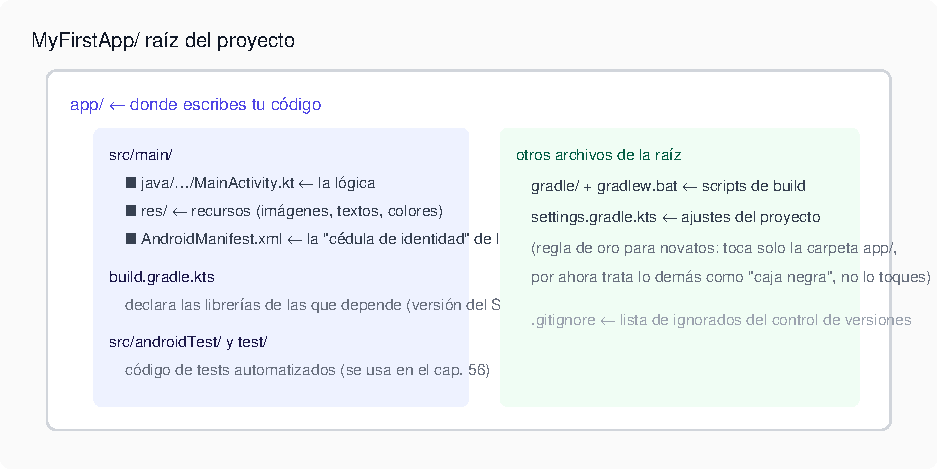
\includegraphics[width=0.92\linewidth]{figures/fig-di-si-shi-jiu-zhang-1}
\\[2pt]\small Figura 2: la estructura del proyecto que un principiante debe conocer (regla para recordar: solo se toca la carpeta app/)
\end{center}

\begin{itemize}
  \item MainActivity.kt: la "puerta principal" de la app. Cuando el usuario toca el icono, es lo primero que despierta. En la plantilla actual se encarga de mostrar "Hello Android!".
  \item AndroidManifest.xml: el "registro civil" de la app: declara cómo se llama, qué icono usa, qué pantallas tiene y qué permisos necesita (cámara, ubicación, etc.).
  \item La carpeta res/: el almacén de recursos, donde viven imágenes, iconos, textos y colores. Poner los textos en archivos de recursos en vez de dejarlos clavados en el código es una buena costumbre del desarrollo Android (facilita cambiar de idioma o de tema).
  \item build.gradle.kts: la receta de construcción: declara la versión mínima soportada y de qué bibliotecas se depende (por ejemplo, Compose).
\end{itemize}

\booksection{Primera prueba: cambia “Hello” por tu nombre}

Abre MainActivity.kt y verás el código generado por la plantilla de Compose. Localiza la línea Text(“Hello Android!”), cambia lo que va entre comillas por tu nombre (por ejemplo, Text(“Hola, soy Ana, ¡esta es mi primera app!”)) y pulsa Ctrl+R (Cmd+R en Mac) para volver a ejecutar. A los pocos segundos, tu nombre aparece en el emulador.

\begin{lstlisting}[language=Kotlin]
setContent {
    MyFirstAppTheme {
        Surface(modifier = Modifier.fillMaxSize()) {
            // v cambia aquí por tu propio texto
            Text("¡Hola, Luis! Esta es mi primera app")
        }
    }
}
\end{lstlisting}

Enhorabuena: acabas de completar un ciclo entero de “cambiar código compilar instalar ejecutar”. Ese ciclo será el pan de cada día del desarrollo. Aprovecha la racha y prueba a cambiar algo más: sube el tamaño de la letra, cambia el color; en el próximo capítulo descubrirás de dónde sale esa “magia”.

\booksection{Primeros auxilios con errores habituales: la “sala de urgencias” de tus dos primeras semanas}

Montando el entorno y durante la primera compilación es muy probable que te cruces con estos tres errores. Tranquilo: todos tienen antídoto:

\begin{center}
\begin{tabularx}{\linewidth}{|X|X|X|}
\hline
\textbf{Síntoma del error} & \textbf{Causa habitual} & \textbf{Antídoto} \tabularnewline
\hline
Gradle sync failed / descarga lenta de dependencias & Mala conexión con los repositorios & Configura en Gradle repositorios espejo (por ejemplo, los mirrors maven de Alibaba Cloud o Tencent Cloud); busca en internet "gradle mirror china" y aplica los cambios \tabularnewline
Faltan componentes del SDK & Se saltó la descarga del SDK al instalar & Settings SDK Manager: instala las plataformas y herramientas que falten \tabularnewline
El emulador no arranca / se queda en negro & Virtualización sin activar o imagen dañada & Activa VT-x/AMD-V en la BIOS; borra el emulador y créalo de nuevo; o pasa directamente a depurar en dispositivo real \tabularnewline
\hline
\end{tabularx}
\end{center}

\begin{center}\small\color{gray}Tabla de urgencias de errores de entorno para principiantes\end{center}

\begin{tcbinfo}{Consejo: la metodología para buscar errores}
La primera línea del mensaje de error es la más valiosa: cópiala tal cual en el buscador y añade la palabra clave “android studio”. No busques preguntas tan genéricas como “no consigo montar el entorno”; busca errores concretos como “Gradle sync failed: Could not resolve com.android.tools.build”. Solo las preguntas exactas reciben respuestas exactas.

\end{tcbinfo}

\begin{tcbpractice}{Manos a la obra: completa tu lista de "ritos de desarrollador"}
(1) Instala Android Studio y deja funcionando el emulador; (2) ejecuta tu app una vez en un dispositivo real y guarda una captura de recuerdo; (3) cambia el texto Hello por tu nombre; (4) comprime el proyecto y guárdalo. Con los cuatro pasos hechos ya puedes anunciar a tus contactos: yo también soy desarrollador Android (con captura como prueba).

\end{tcbpractice}

\begin{tcbsummary}{Resumen del capítulo}
\begin{itemize}
  \item Android Studio = el IDE oficial y gratuito; se recomiendan 16 GB de RAM + 20 GB de disco + virtualización activada
  \item Los tres imprescindibles de un proyecto nuevo: nombre, nombre de paquete (único en el mundo, no publiques con com.example) y SDK mínimo (desde API 26)
  \item Dos formas de ejecutar: el emulador (un móvil virtual en el ordenador) y el dispositivo real (activa la Depuración por USB y recuerda apagarla al acabar)
  \item La regla del proyecto: solo se toca la carpeta app/: MainActivity.kt es la puerta principal, el Manifest el registro civil y res/ el almacén de recursos
  \item El día a día del desarrollo = cambiar código Run ver el resultado, una y otra vez
\end{itemize}

\end{tcbsummary}
